\documentclass[a4paper]{article}
\usepackage{polski}
\usepackage[utf8]{inputenc}
\usepackage{enumerate}
\usepackage{graphicx}
\usepackage{float}
\usepackage{indentfirst}  % załatwia to problem z brakiem wciąć na początku sekcji

\usepackage{geometry}
\newgeometry{tmargin=2.5cm, bmargin=2cm, lmargin=2cm, rmargin=2cm}

\title{Założenia projektowe, specyfikacja funkcjonalna, kryteria ewaluacji}
\date{}
\author{}

\begin{document}
\maketitle



\section{Dekompozycja układu mechanicznego i elektronicznego:} 
\begin{figure}[H]
\centering
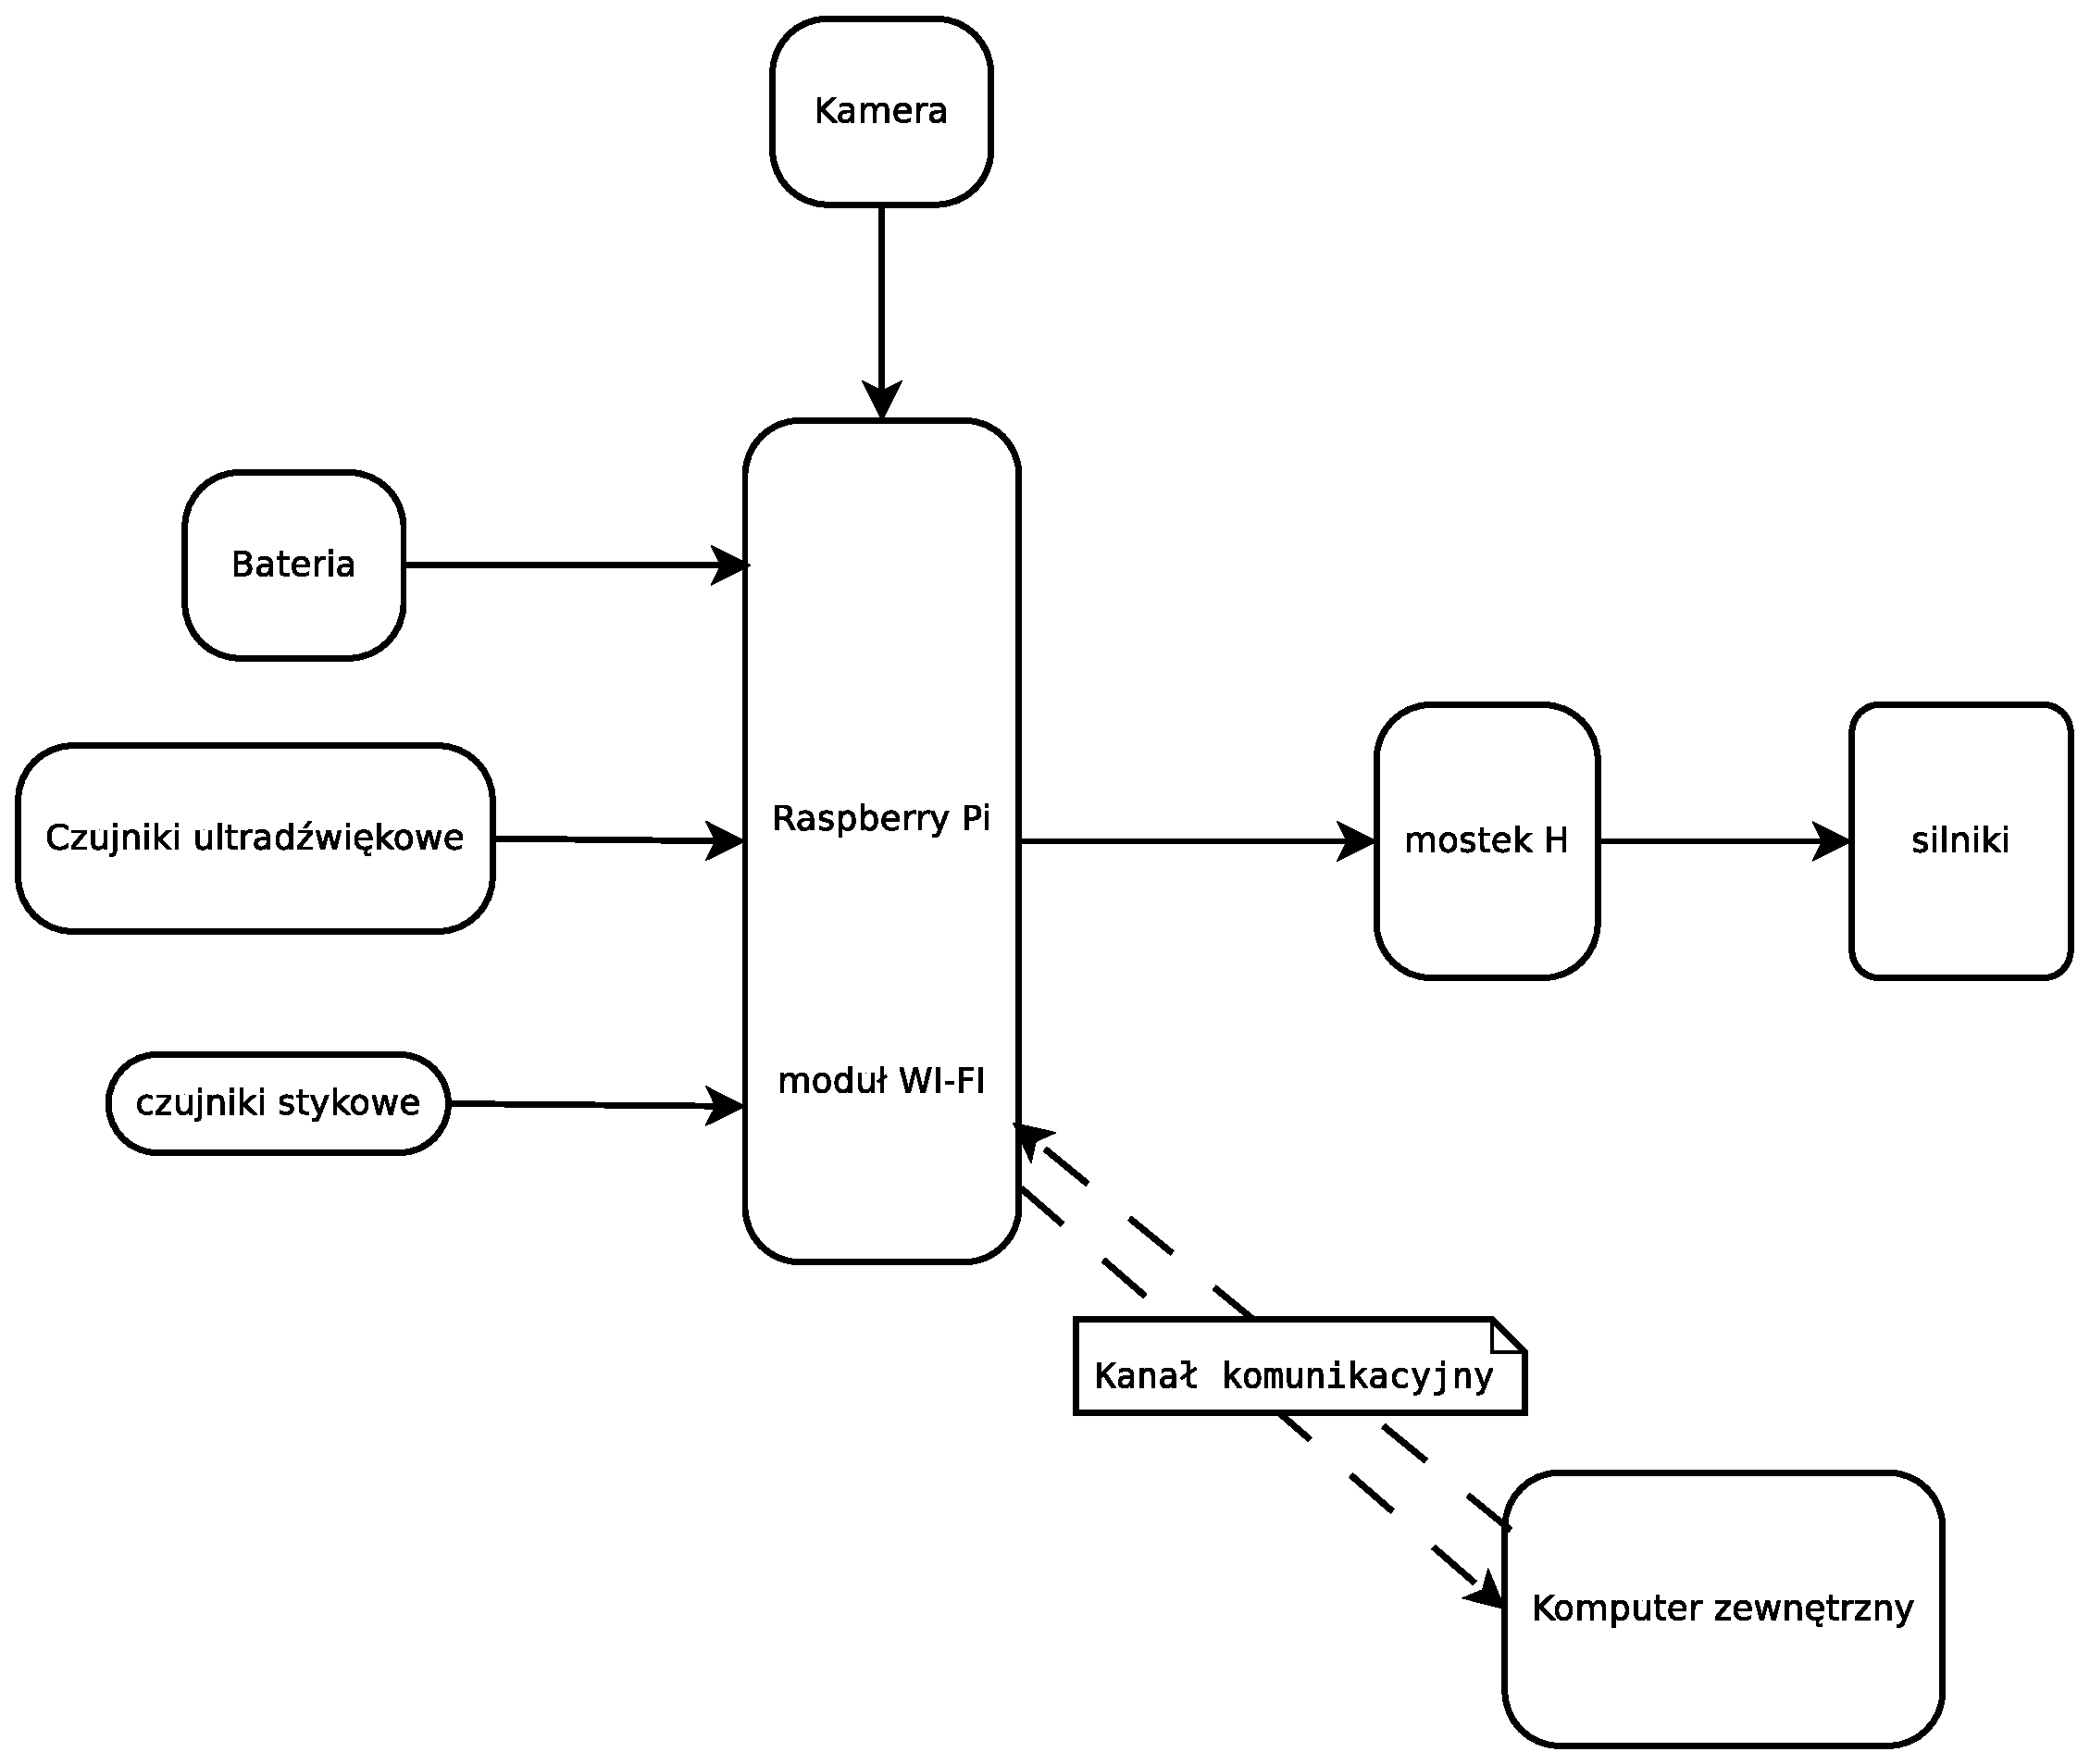
\includegraphics[width=15cm]{idea_sprzet-mech.eps}
\caption{Schemat ideowy ilustrujący zależności między komponentami}
\end{figure}

\section{Dekompozycja oprogramowania:}
\begin{figure}[H]
\centering
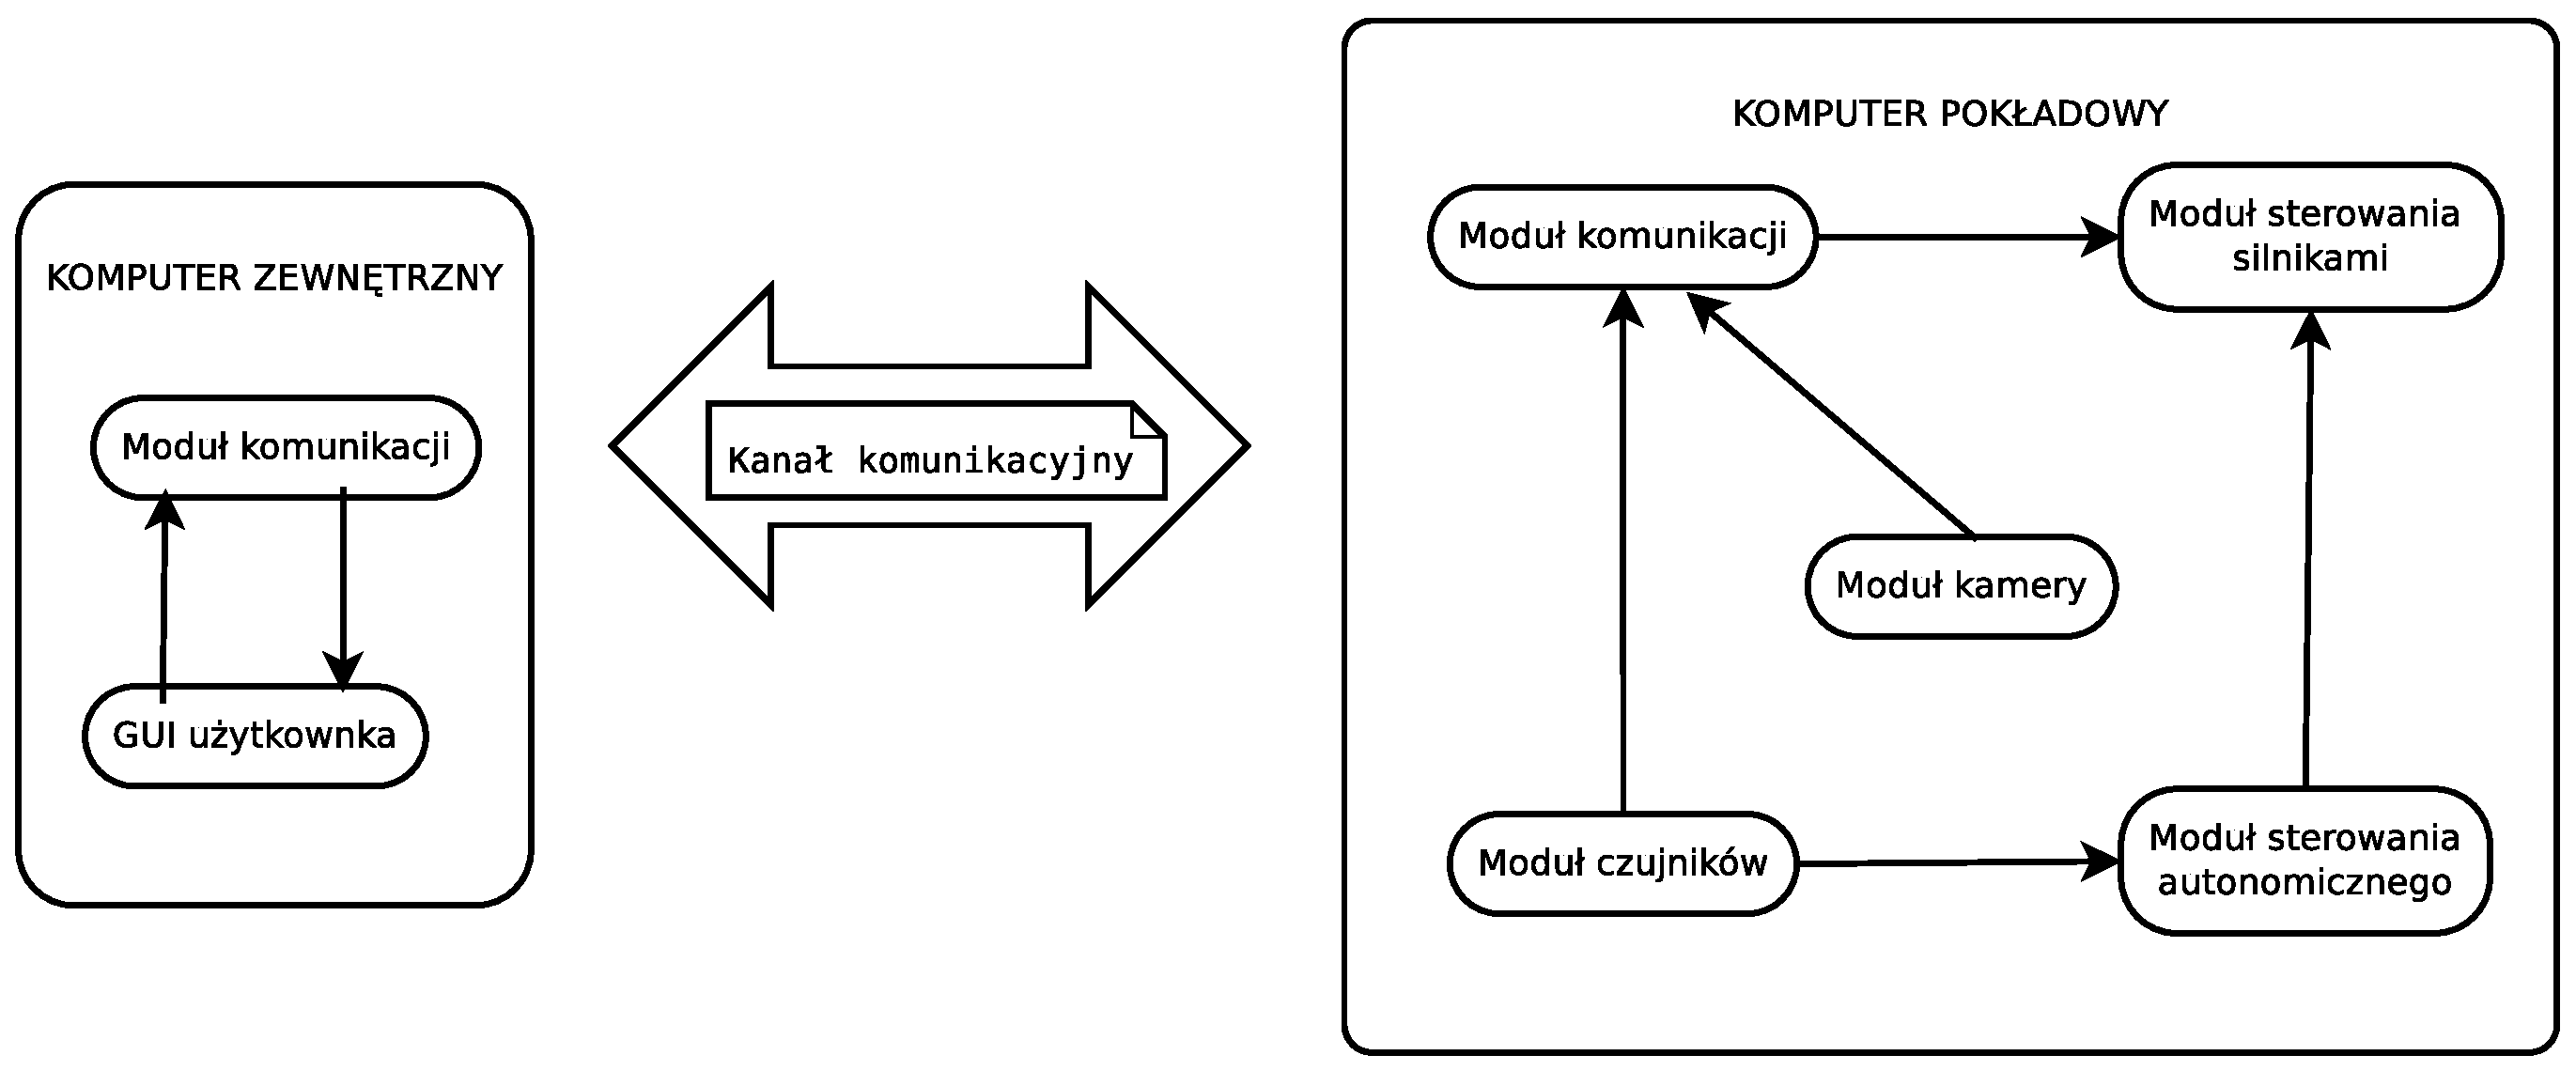
\includegraphics[width=15cm]{idea_programowa.eps}
\caption{Schemat ideowy ilustrujący zależności między komponentami części programowej}
\end{figure}

\section{Opis komponentów:}

\subsection{Komponenty elektroniczno - mechaniczne:}


Bateria - komponent odpowiedzialny za dostarczanie energii elektrycznej zasilającej Raspberry Pi oraz silniki o następujących paramterach:
\begin{itemize}
\item Typ baterii Ni-MH (niklowo-metalowo-wodorkowy)
\item Napięcie nominalne 8,4 V
\item Pojemność 12000 mAh
\end{itemize}


Czujniki ultradźwiękowe - czujniki zbliżeniowe odpowiedzialne za wykrywanie przeszkód za pomocą fal ultradźwiękowych i wysyłanie odczytów do Raspberry. Czujniki ultradźwiękowe o parametrach:
\begin{itemize}
\item Napięcie zasilania: 5 V
\item Średni pobór prądu: 15 mA
\item Zakres pomiarowy: od 2 cm do 200 cm
\item Wyjście: sygnał częstotliwościowy
\item Częstotliwość pracy: 40 kHz
\end{itemize}
Czujniki stykowe - czujniki zbliżeniowe odpowiedzialne za wykrywanie przeszkód za pomocą styków, jest to opcja ostatecznego zatrzymania układu w przypadku, gdy przeszkody nie zostanie wykryte przez czujniki ultradźwiękowe - o parametrach:
\begin{itemize}
\item Napięcie pracy: maks. 250 V
\item Natężenie prądu: maks. 5 A
\item Liczba wyprowadzeń: 3 (C, NO, NC)
\end{itemize}
Kamera - komponent odpowiedzialny za przekazywanie obrazu otoczenia do Raspberry - o parametrach:
\begin{itemize}
\item Kamera zgodna z Raspberry Pi w wersji 3, 2, B+, A+ oraz starszych A i B
\item Matryca: 5 MPx
\item Czujnik: OV5647
\item Matryca CCD: 1/4"
\item Kąt widzenia - przekątna: 75,7 stopni
\item Przesłona: 2,0
\item Ogniskowa: 6 mm (zmienna)
\item Posiada 4 otwory montażowe
\item Wymiary: 32 x 32 mm
\end{itemize}
Mostek H - układ elektroniczny umożliwiający zmianę kierunku obrotu silnika prądu stałego przez,,odwracanie" biegunów zasilania - o parametrach:
\begin{itemize}
\item Maksymalne napięcie zasilania silników: 36 V
\item Średni prąd kanał: 0,6 A
\item Szczytowy prąd na kanał: 1,2 A
\item Obudowa: DIP 16 (przewlekana)
\item Wbudowane diody zabezpieczające
\end{itemize}
Silniki i koła - komponenty odpowiedzialne za ruch robota w zależności od otrzymanych sygnałów.
Wykorzystanie mostka H umożliwia pracę silnika w dwóch kierunkach. Parametry silników i kół:

\begin{enumerate}
\item Parametry silnika
\begin{itemize}
\item Napięcie zasilania: 5 V
\item Pobór prądu: ok. 180 mA
\item Zintegrowana przekładnia: 48:1
\item Obustronny wał
\item Prędkość obrotowa po przekładni: ok. 80 obr/min
\item Moment obrotowy po przekładni: ok. 0,5 kg*cm (0,049 Nm)
\end{itemize}

\item Parametry koła
\begin{itemize}
\item Średnica opony: 65 mm
\item Szerokość opony: 26 mm
\end{itemize}
\end{enumerate}

\subsection{Komponenty programowe:}
GUI użytkownika:
\begin{itemize}
\item przeznaczenie: Służy jako interfejs człowiek-maszyna
\item funkcjonalności: GUI wyświetla obraz z kamery robota oraz dane sensoryczne robota. Pozwala również użytkownikowi na wydawanie rozkazów sterujących. 
\end{itemize}

Moduł komunikacji:
\begin{itemize}
\item przeznaczenie: Zapewnie połączenie między komuterem zewnętrznym a pokładowym
\item funkcjonalności: Poprzez kanał komunikacyjny przesyłany jest obraz z kamery oraz dane sensoryczne (w jedną stroną), a także rozkazy użytkownika (w drugą stronę). 
\end{itemize}

Moduł kamery:
\begin{itemize}
\item przeznaczenie: Obsługa kamery
\item funkcjonalności: Moduł pozyskuje obraz z kamery, dokonuje ewentualnej kompresji oraz przesyła dane do modułu komunikacji
\end{itemize}

Moduł sterowania silnikami:
\begin{itemize}
\item przeznaczenie: Zamiania otrzymanych rozkazów na odpowiednią sekwensję ruchów silników
\item funkcjaonalności: Dane wejściowe modułu to polecenia dotyczące ruchu całego robota. Na ich podstawie moduł generuje sygnały wyjściowe decydujące o tym które silniki mają się poruszać, i z jaką prędkością (generowanie kanałów PWM). 
\end{itemize}
\newpage
Moduł czujników:
\begin{itemize}
\item przeznaczenie: Pozyskiwanie informacji o otoczeniu robota
\item funkcjonalności: Moduł dokonuje co niewielką chwilę czasu pomiaru odległości od otoczenia za pomocą czujników ultradźwiękowych. Oprócz tego reaguje na naciśnięcie czujników stykowych (micro switch)
\end{itemize}

Moduł sterowania autonomicznego:
\begin{itemize}
\item przeznaczenie: Niezależne od użytkownika sterowanie robotem w sytuacjach awaryjnych. 
\item funkcjonalności: Na podstawie danych z czujników moduł podejmuje decyzję o awaryjnym zatrzymaniu robota, kiedy jego dalszy ruch grozi kolizją. Rozkazy tego modułu mają wyższy priorytet od rozkazów użytkownika. 
\end{itemize}

%\section{ Zależności we/wy:} %nie wiem czy to już nie jest umieszczone na diagramach

\section{ Kryteria ewaluacji:}

Robot czterokołowy umożliwi zdalne sterowanie w pomieszczeniu zamkniętym i dokonanie inspekcji pomieszczenia z zapisem video i sygnałów ze wszystkich czujników pomiarowych. Wykrywanie przeszkód odbywa się dwustopniowo: przez analizę danych z czujników ultradźwiękowych, oraz przez analizę danych odebranych z czujników stykowych. Po wykryciu przeszkody robot spróbuje ominąć przeszkodę. W razie braku możliwości ominięcia przeszkody robot zatrzyma się.

\section{ Baza sprzętowa i programowa:}
Komputer pokładowy:
\begin{itemize}
\item Płytka uruchomieniowa: Raspberry Pi 3 model B
\item System operacyjny:     Raspbian GNU/Linux 8.0 (jessie)
\item Kompilator:            gcc 4.9.2
\item Framework robotyczny:  ROS indigo 1.11.16
\end{itemize}

Komputer zewnętrzny:
\begin{itemize}
\item System operacyjny:     Ubuntu 14.04.4 LTS (trusty)
\item Kompilator:            gcc 4.8
\item Framework robotyczny:  ROS indigo 1.11.16
\end{itemize}


\end{document}